\begin{figure*}[ht]

\begin{center}

\scalebox{0.6}{





\tikzset{every picture/.style={line width=0.75pt}} %set default line width to 0.75pt        

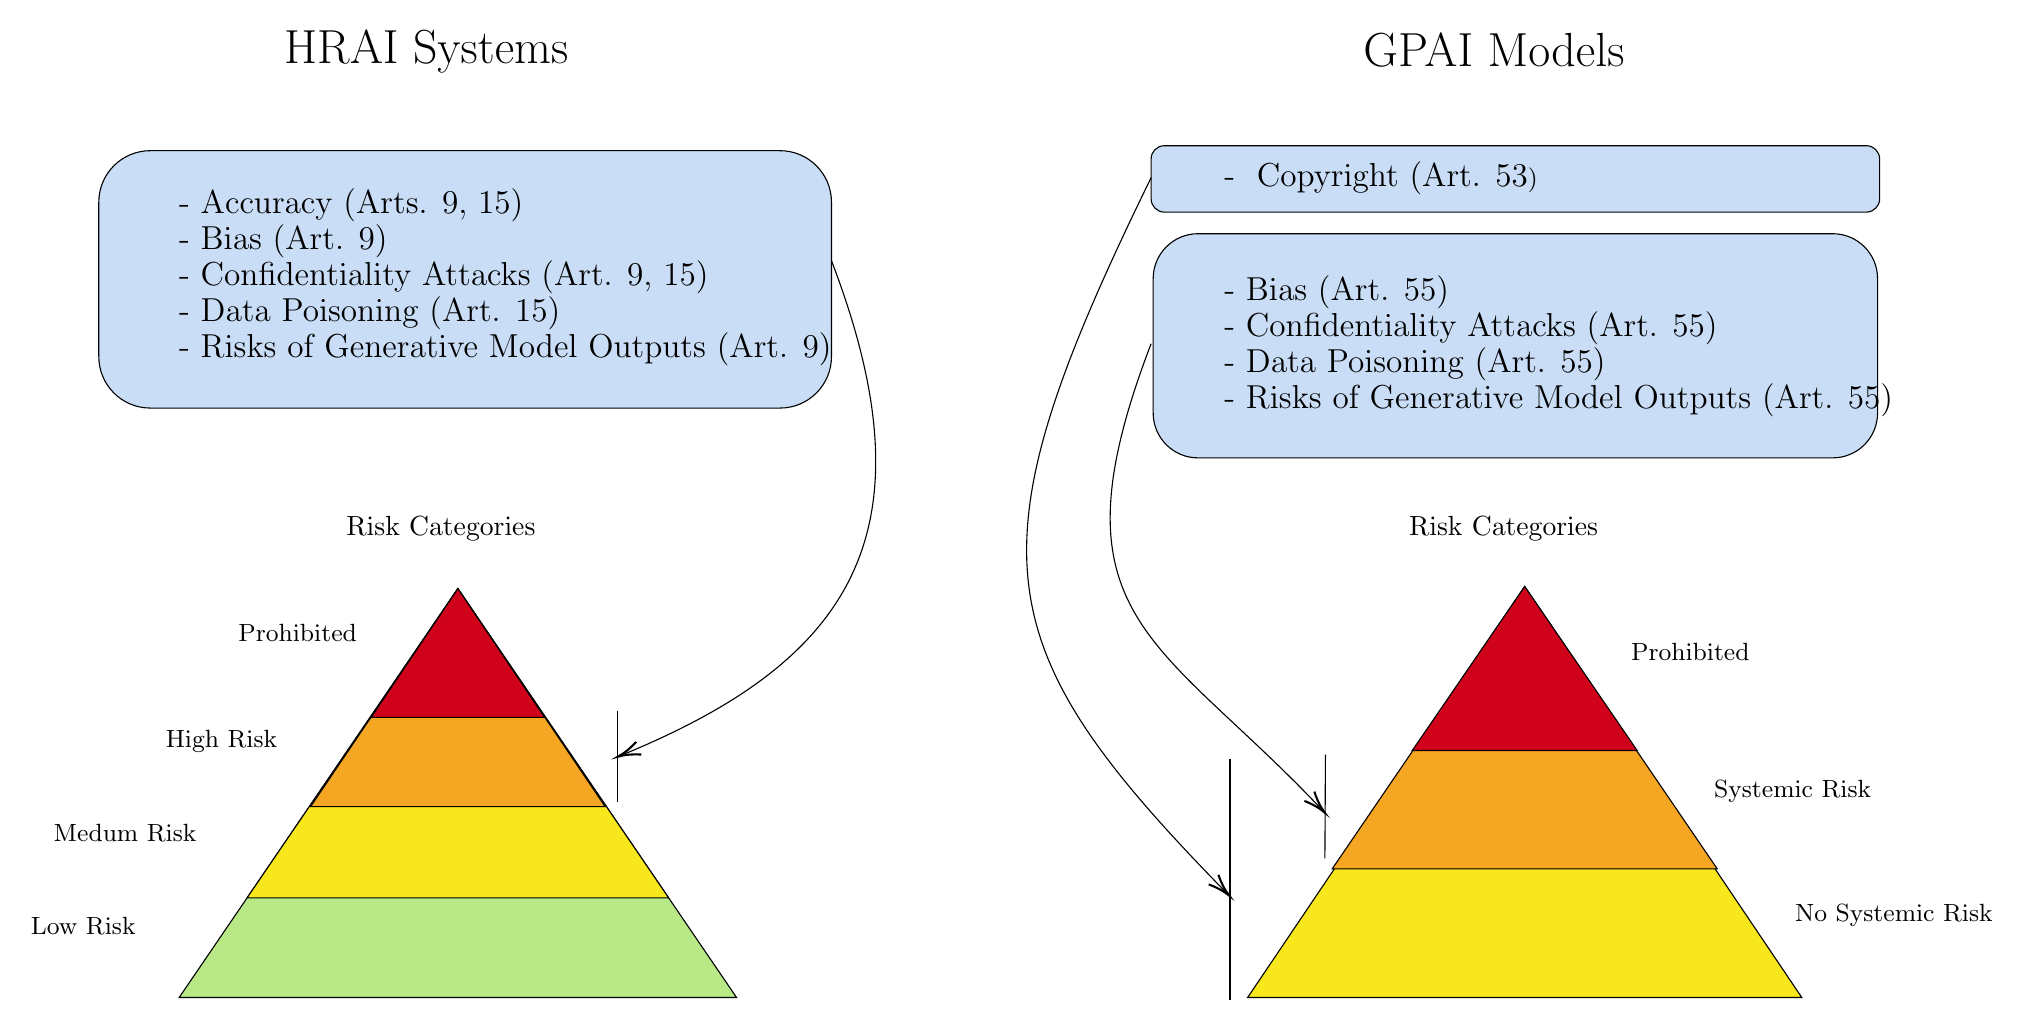
\begin{tikzpicture}[x=0.75pt,y=0.75pt,yscale=-1,xscale=1]
%uncomment if require: \path (0,592); %set diagram left start at 0, and has height of 592

%Shape: Triangle [id:dp5428005874858406] 
\draw  [fill={rgb, 255:red, 184; green, 233; blue, 134 }  ,fill opacity=1 ] (234,341) -- (368.28,538) -- (99.72,538) -- cycle ;
%Shape: Triangle [id:dp3047849031551493] 
\draw  [fill={rgb, 255:red, 248; green, 231; blue, 28 }  ,fill opacity=1 ] (748,340) -- (881.5,538) -- (614.5,538) -- cycle ;
%Shape: Triangle [id:dp0818620622382471] 
\draw  [fill={rgb, 255:red, 245; green, 166; blue, 35 }  ,fill opacity=1 ] (748,340) -- (840.75,476) -- (655.25,476) -- cycle ;
%Shape: Triangle [id:dp7631457704181537] 
\draw  [fill={rgb, 255:red, 208; green, 2; blue, 27 }  ,fill opacity=1 ] (748,340) -- (802.19,419) -- (693.81,419) -- cycle ;
%Shape: Triangle [id:dp7055596435513258] 
\draw  [fill={rgb, 255:red, 248; green, 231; blue, 28 }  ,fill opacity=1 ] (234,341) -- (335.56,490) -- (132.44,490) -- cycle ;
%Shape: Triangle [id:dp9202964178531197] 
\draw  [fill={rgb, 255:red, 245; green, 166; blue, 35 }  ,fill opacity=1 ] (234,341) -- (304.94,446) -- (163.06,446) -- cycle ;
%Shape: Triangle [id:dp09535399425331859] 
\draw  [fill={rgb, 255:red, 208; green, 2; blue, 27 }  ,fill opacity=1 ] (234,341) -- (275.77,403) -- (192.23,403) -- cycle ;
%Rounded Rect [id:dp25406852669435454] 
\draw  [fill={rgb, 255:red, 201; green, 221; blue, 246 }  ,fill opacity=1 ] (61,154.8) .. controls (61,141.1) and (72.1,130) .. (85.8,130) -- (389.2,130) .. controls (402.9,130) and (414,141.1) .. (414,154.8) -- (414,229.2) .. controls (414,242.9) and (402.9,254) .. (389.2,254) -- (85.8,254) .. controls (72.1,254) and (61,242.9) .. (61,229.2) -- cycle ;
%Rounded Rect [id:dp6638236112064699] 
\draw  [fill={rgb, 255:red, 201; green, 221; blue, 246 }  ,fill opacity=1 ] (569,191.6) .. controls (569,179.67) and (578.67,170) .. (590.6,170) -- (896.4,170) .. controls (908.33,170) and (918,179.67) .. (918,191.6) -- (918,256.4) .. controls (918,268.33) and (908.33,278) .. (896.4,278) -- (590.6,278) .. controls (578.67,278) and (569,268.33) .. (569,256.4) -- cycle ;
%Curve Lines [id:da6560168607616261] 
\draw    (414,183) .. controls (464.75,315.34) and (422.43,376.39) .. (312.66,421.32) ;
\draw [shift={(311,422)}, rotate = 337.93] [color={rgb, 255:red, 0; green, 0; blue, 0 }  ][line width=0.75]    (10.93,-3.29) .. controls (6.95,-1.4) and (3.31,-0.3) .. (0,0) .. controls (3.31,0.3) and (6.95,1.4) .. (10.93,3.29)   ;
%Straight Lines [id:da5242356218911126] 
\draw    (311,400) -- (311,444) ;
%Rounded Rect [id:dp6795269102209953] 
\draw  [fill={rgb, 255:red, 201; green, 221; blue, 246 }  ,fill opacity=1 ] (568,134) .. controls (568,130.47) and (570.87,127.6) .. (574.4,127.6) -- (912.6,127.6) .. controls (916.13,127.6) and (919,130.47) .. (919,134) -- (919,153.2) .. controls (919,156.73) and (916.13,159.6) .. (912.6,159.6) -- (574.4,159.6) .. controls (570.87,159.6) and (568,156.73) .. (568,153.2) -- cycle ;
%Straight Lines [id:da5998648988158835] 
\draw    (606,423) -- (606,539) ;
%Curve Lines [id:da489843699645353] 
\draw    (568,223) .. controls (517.26,355.34) and (571.45,363.92) .. (650.54,447.73) ;
\draw [shift={(651.73,449)}, rotate = 226.83] [color={rgb, 255:red, 0; green, 0; blue, 0 }  ][line width=0.75]    (10.93,-3.29) .. controls (6.95,-1.4) and (3.31,-0.3) .. (0,0) .. controls (3.31,0.3) and (6.95,1.4) .. (10.93,3.29)   ;
%Straight Lines [id:da4800745204547854] 
\draw    (652,421) -- (651.73,471) ;
%Curve Lines [id:da31844169520160337] 
\draw    (568,143) .. controls (479,325) and (487,368) .. (605.73,489) ;
\draw [shift={(605.73,489)}, rotate = 225.54] [color={rgb, 255:red, 0; green, 0; blue, 0 }  ][line width=0.75]    (10.93,-3.29) .. controls (6.95,-1.4) and (3.31,-0.3) .. (0,0) .. controls (3.31,0.3) and (6.95,1.4) .. (10.93,3.29)   ;

% Text Node
\draw (691,305) node [anchor=north west][inner sep=0.75pt]  [font=\normalsize] [align=left] {Risk Categories};
% Text Node
\draw (798,366) node [anchor=north west][inner sep=0.75pt]  [font=\small] [align=left] {Prohibited};
% Text Node
\draw (838,432) node [anchor=north west][inner sep=0.75pt]  [font=\small] [align=left] {Systemic Risk};
% Text Node
\draw (877,492) node [anchor=north west][inner sep=0.75pt]  [font=\small] [align=left] {No Systemic Risk};
% Text Node
\draw (179,305) node [anchor=north west][inner sep=0.75pt]  [font=\normalsize] [align=left] {Risk Categories};
% Text Node
\draw (127,357) node [anchor=north west][inner sep=0.75pt]  [font=\small] [align=left] {Prohibited};
% Text Node
\draw (92,408) node [anchor=north west][inner sep=0.75pt]  [font=\small] [align=left] {High Risk};
% Text Node
\draw (27,498) node [anchor=north west][inner sep=0.75pt]  [font=\small] [align=left] {Low Risk};
% Text Node
\draw (38,453) node [anchor=north west][inner sep=0.75pt]  [font=\small] [align=left] {Medum Risk};
% Text Node
\draw (98.4,147) node [anchor=north west][inner sep=0.75pt]  [font=\scriptsize] [align=left] {{\large - Accuracy (Arts. 9, 15)}\\{\large - Bias (Art. 9)}\\{\large - Confidentiality Attacks (Art. 9, 15)}\\{\large - Data Poisoning (Art. 15)}\\{\large - Risks of Generative Model Outputs (Art. 9)}};
% Text Node
\draw (602,189) node [anchor=north west][inner sep=0.75pt]  [font=\scriptsize] [align=left] {{\large - Bias (Art. 55)}\\{\large - Confidentiality Attacks (Art. 55)}\\{\large - Data Poisoning (Art. 55)}\\{\large - Risks of Generative Model Outputs (Art. 55)}};
% Text Node
\draw (149,71) node [anchor=north west][inner sep=0.75pt]  [font=\LARGE] [align=left] {HRAI Systems};
% Text Node
\draw (669,72) node [anchor=north west][inner sep=0.75pt]  [font=\LARGE] [align=left] {GPAI Models};
% Text Node
\draw (602.03,134) node [anchor=north west][inner sep=0.75pt]  [font=\scriptsize] [align=left] {{\large - \ Copyright (Art. 53}{\small )}};


\end{tikzpicture}

}

\end{center}
\caption{\textit{\textbf{AIA Uses Cases for Machine Unlearning.}}\label{fig:pyramids}}
\end{figure*}